\section{Alternating Bit Protocol - Modelling, Specification and Verification}
% no \IEEEPARstart
The alternating bit protocol is a simple yet effective protocol (usually used as a test case), designed to ensure reliable communication through unreliable transmission mediums, and it is used for managing the retransmission of lost messages \cite{ReactiveSystems3}\cite{Kulick}.

The representation of Alternating Bit Protocol (hereby abbreviated as ABP) is shown bellow, and it consists of a $Sender$ $S$, a $Receiver$ $R$ and two channels $Transport$ $T$ and $Acknowledge$ $A$. 

\begin{figure}[!ht]
\centering
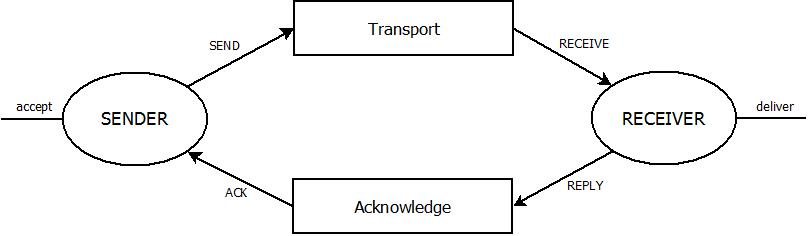
\includegraphics[width=4.5in]{abp}
\caption{Alternating bit protocol}
\label{fig:abp}
\end{figure}

All of the transitions in the ABP are internal synchronization and the only visible transitions are deliver and accept, which can occur only sequentially. 

The specication of $ABP$ is that it should act as a simple buffer, as follows:\\
$ABP=\overline{deliver}.accept.ABP$

Messages are sent from a sender $S$ to a receiver $R$. Channel from $S$ to $R$ is initialized and there are no messages in transit. There is no direct communication between the sender $S$ and the receiver $R$, and all messages must travel trough the medium (transport and acknowledge channel). The ABP works like this:
\begin{enumerate}
	\item Each message sent by $S$ contains the protocol bit, 0 or 1.\\
	      Here is the implementation:\\
	      $Imp \stackrel{def}{=}\left(S|T|R|A\right)\backslash L$, \\
	      where $L = \left(send0,send1,receive0,receive1,reply0,reply1,ack0,ack1\right)$ is the set of restricted actions.
	\item When a sender $S$ sends a message, it sends it repeatedly (with its corresponding bit) until receiving an acknowledgment ($ack0$ or $ack1$) from a receiver $R$ that contains the same protocol bit as the message being sent.\\
	      $S=\overline{send0}.S+ack0.accept.S_{1}+ack1.S$\\
	      $S_{1}=\overline{send1}.S_{1}+ack1.accept.S+ack0.S_{1}$\\
	      The transport channel transmits the message to the receiver, but it may lose the message (lossy channel) or transmit it several times (chatty channel).
	      $T=send0.\left(T+T_{1}\right)+send1.\left(T+T_{2}\right)$\\
	      $T_{1}=\overline{receive0}.\left(T+T_{1}\right)$\\
	      $T_{2}=\overline{receive1}.\left(T+T_{2}\right)$
  \item When $R$ receives a message, it sends a reply to $S$ that includes the protocol bit of the message received. When a message is received for the first time, the receiver delivers it for processing, while subsequent messages with the same bit are simply acknowledged.
        $R=receive0.\overline{deliver}.R_{1}+\overline{reply1}.R+receive1.R$\\
        $R_{1}=receive1.\overline{deliver}.R+\overline{reply0}.R_{1}+receive0.R_{1}$\\
        Again the acknowledgement channel sends the ack to sender, and it also can acknowledge it several times or lose it on the way to the sender.\\
        $A=reply0.\left(A+A_{1}\right)+reply1.\left(A+A_{2}\right)$\\
        $A_{1}=\overline{ack0}.\left(A+A_{1}\right)$\\
        $A_{2}=\overline{ack1}.\left(A+A_{2}\right)$
  \item When $S$ receives an acknowledgment containing the same bit as the message it is currently transmitting, it stops transmitting that message, flips the protocol bit, and repeats the protocol for the next message.\cite{Kulick}\cite{ProcessAlgebraParallel}
\end{enumerate}

In order to verify the alternating bit protocol, it needs to be proven that the
implementation meets its specification, or more precisely it needs to be shown
that $ABP\approx Imp$. Such a bisimulation $R$ can be found as follows:

\begin{table}
\begin{tabular}{| p{6.5cm} | p{3.5cm} | }
	
  \hline                       
	ABP implementation states &
	ABP specification states
	\\ \hline
	
$\left(S|T|R|A\right)\backslash L$,\\
$\left(S|\left(T+T1\right)|R|A\right)\backslash L$,\\
$\left(S|\left(T+T1\right)|R|\left(A+A2\right)\right)\backslash L$,\\
$\left(S|T|R|\left(A+A2\right)\right)\backslash L$,\\
$\left(S|\left(T+T1\right)|\overline{deliver}.R1|A\right)\backslash L$,\\
$\left(S|\left(T+T1\right)|\overline{deliver}.R1|\left(A+A2\right)\right)\backslash L$,\\
$\left(S1|\left(T+T1\right)|R1|\left(A+A1\right)\right)\backslash L$,\\
$\left(S1|\left(T+T2\right)|\overline{deliver}.R|\left(A+A1\right)\right)\backslash L$,\\
$\left(S1|\left(T+T2\right)|R1|\left(A+A1\right)\right)\backslash L$,\\
$\left(S|\left(T+T2\right)|R|\left(A+A2\right)\right)\backslash L$\\ &
  $ABP$   
  \\ \hline
   
$\left(accept.S1|\left(T+T1\right)|R1|\left(A+A1\right)\right)\backslash L$,\\ 
$\left(S|\left(T+T1\right)|R1|\left(A+A1\right)\right)\backslash L$,\\
$\left(S|\left(T+T1\right)|R1|\left(A+A2\right)\right)\backslash L$,\\
$\left(S|\left(T+T1\right)|R1|A\right)\backslash L$,\\
$\left(S1|\left(T+T2\right)|R|\left(A+A2\right)\right)\backslash L$,\\
$\left(accept.S|\left(T+T2\right)|R|\left(A+A2\right)\right)\backslash L$,\\
$\left(S1|\left(T+T2\right)|R|\left(A+A1\right)\right)\backslash L$\\ &
  $ABP'$
  \\ \hline  
\end{tabular}
\\
\caption{Verification of Alternating Bit Protocol}
\label{table3}
\end{table}
